\chapter{Improvements in the Analysis}

In the previous chapter, we had show examples where the heap liveness analysis applied to the synchronized control flow graph returned a highly-over approximated access graph. The reason for this being the inter-thread synchronization edges not being treated differently from intra-thread edges. There is also a need to ensure that the final data flow value obtained can actually be a result of valid program execution. \\

In order to achieve this we need to analyze critical sections in all the threads. An intra-thread analysis will be required to be performed. We need to figure out the whether there exists a loop outside the critical section. If there is no such loop then we can say that the critical section will be executed once. Otherwise, The critical section can be executed zero or more times. Note that this information in thread independent. Once we have the thread dependent information , we can add inter-thread edges. The edges will only be triggered based on the condition that checks if the critical section can be executed. The condition would involve comparing counters of the number of times a critical section is executed. \\

One way to achieve this is to label the edges with the number of times the transition is possible. Considering the examples in the last chapter figure 5.1, 5.2 and 5.3, we can suggest the following access graphs at the statement main(). See figure 6.1. \\


\begin{figure}
	\centering
	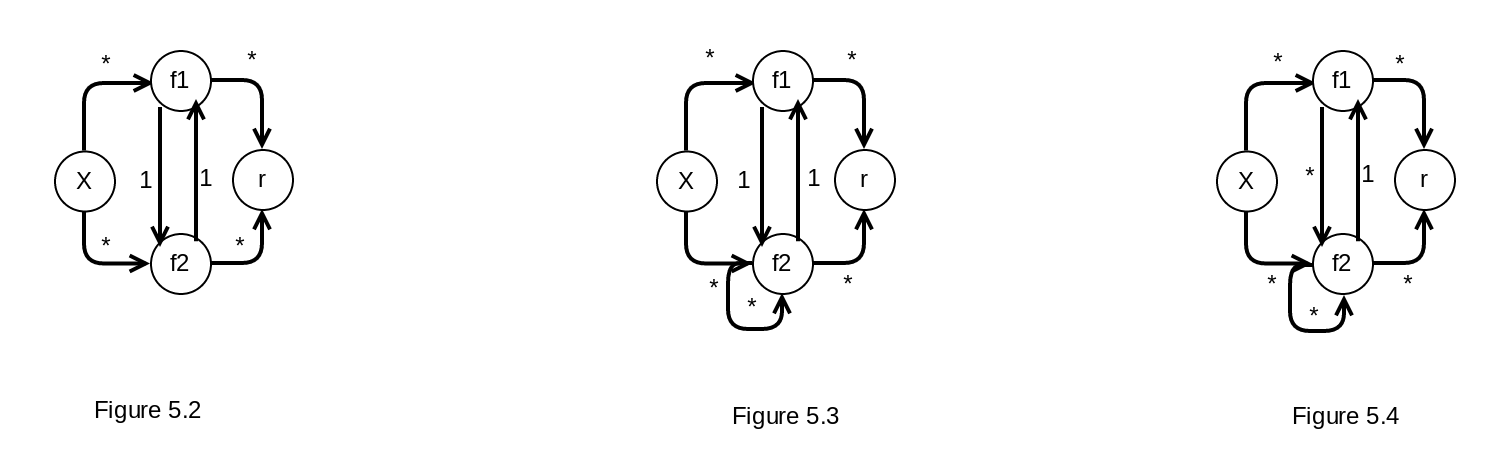
\includegraphics[width=0.8\textwidth]{Figures/access_graph_rep.png}
	\caption{Desired Access graphs for fig 5.2,5.3 and 5.4}
	\label{fig:ch5example}
\end{figure}
 
In examples 5.2,5,3 and 5.4 , we had observed that access graph at the statement main() was the same. We now display the desired representation of access graph. For example 5.2, we have observed that the critical section can only be executed once for both the threads. So we need to mark the edge with either 1 or *, where 1 denotes that the transition can only be performed once and * is a doesn't care condition. \\

For 5.3, we had a loop inside critical section of thread 2. However the critical section could only be executed once. There will be a self loop around $f_2$ in the access graph. The edges from $f_1$ and $f_2$ are representative of a thread change. Since there are no loops across/outside the critical section, we can conclude that both these will execute once and mark the two edges 1. \\

For example 5.4, there is a thread 2 has a loop across the lock and unlock section. Thus now the edge representing transition from $C_1$ to $C_2$ can be executed any number of times. The desired access graph for 5.4, should be the similar to 5.3 except for the edge from $f_1$ to $f_2$ being labeled as * instead of 1. \\

We may need to modify the analysis in order to obtain the desired access graph for all the examples. One way may be to change the way we merge and summarize access graphs different threads. Another way could be   

\section{Concurrent Heap Access examples}

Let us try to understand the how heap memory is actually accessed by threaded programs using shared memory. This will be better understood by taking up the example of a concurrent data structure say tree. Each node of the tree has \emph{l} and \emph{r} fields pointing to children and a \emph{data} field. \\

Consider the simplest example for this, similar to example 5.2 in figure 6.2. The access pattern is either $T_1$ followed by $T_2$ or the reverse. If $T_1$ is executed first then the object \emph{x.l.r} is accessed otherwise \emph{x.r.l} is accessed. This corresponds to the iteration 1 of simple concurrent heap liveness analysis. (See figure 4.4) So if the analysis is stopped at this point we would obtain the desired access graph in this case. \\

\begin{figure}
	\centering
	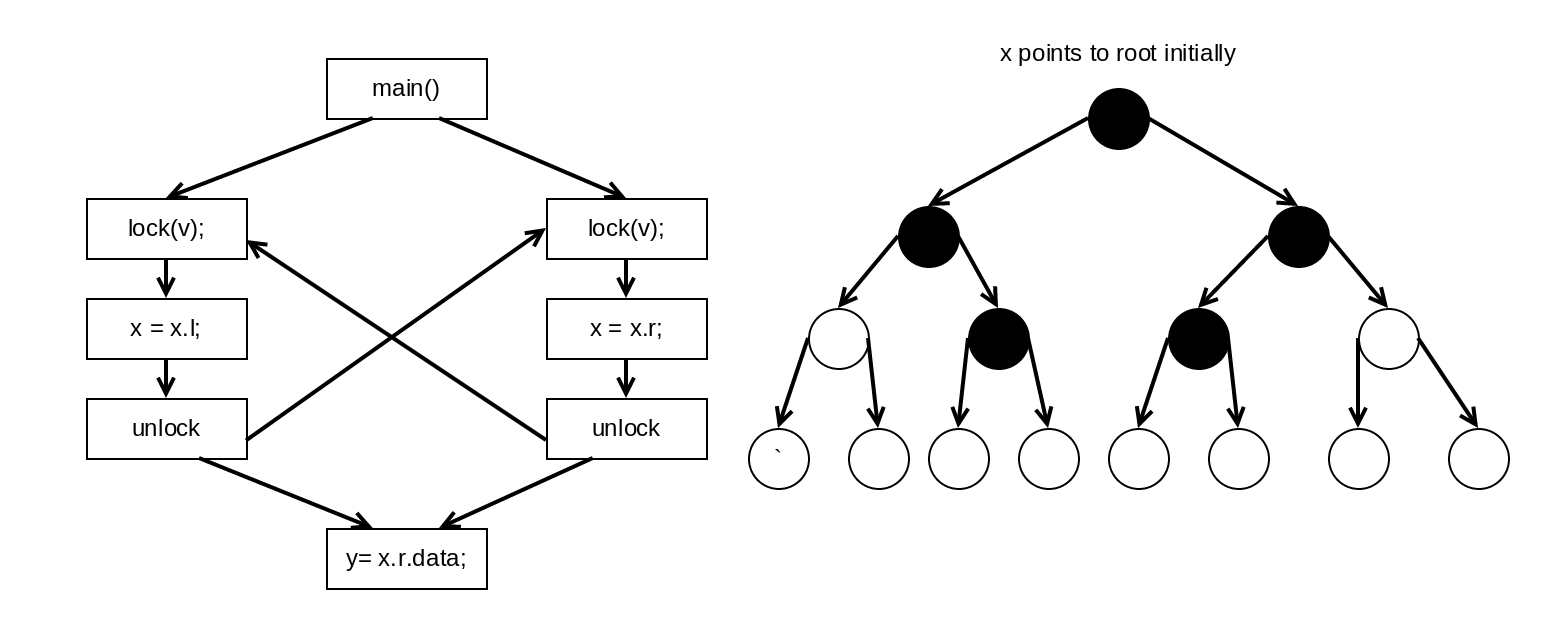
\includegraphics[width=0.8\textwidth]{Figures/tree1.png}
	\caption{Concurrent access example in a tree}
	\label{fig:ch5example}
\end{figure}  

Consider another example with a loop within the critical section in Figure 6.3. This is again inspired from Figure 5.3. Again the access pattern may be either $T_1$ followed by $T_2$ or the reverse. This implies the objects accessed will satisfy the regular expression \emph{x.l.r\textsuperscript{*}} or \emph{x.r\textsuperscript{*}.l} depending on the  starting thread. Figure 6.3 shows the possible nodes that can be accessed by the concurrent program. It just maps the regular expression to the tree topology. \\

\begin{figure}
	\centering
	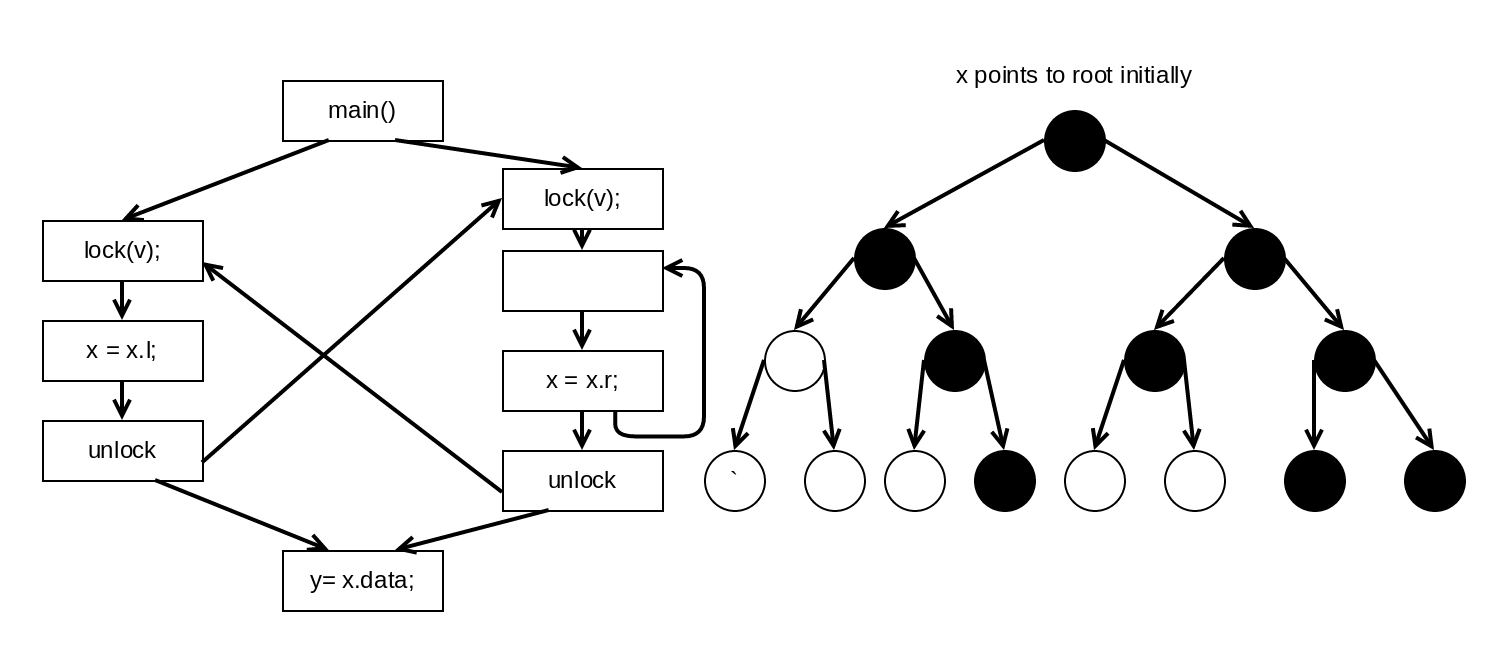
\includegraphics[width=0.8\textwidth]{Figures/tree2.png}
	\caption{Another Concurrent access example in a tree}
	\label{fig:ch5example}
\end{figure}

Now we will look into the possible executions of the example in Figure 6.4. This is the case of presence of loop across critical section. We will have two possible execution orders corresponding to start from $T_1$ or $T_2$ : \emph{x.l.r\textsuperscript{*}}, {x.r\textsuperscript{+}.l.r\textsuperscript{*}}. Looking at the difference between this example and Figure 6.3, we notice that \emph{r\textsuperscript{+}} links from all the nodes of the type \emph{x.r\textsuperscript{+}.l} can be additionally accessed by this program. \\ 

\begin{figure}
	\centering
	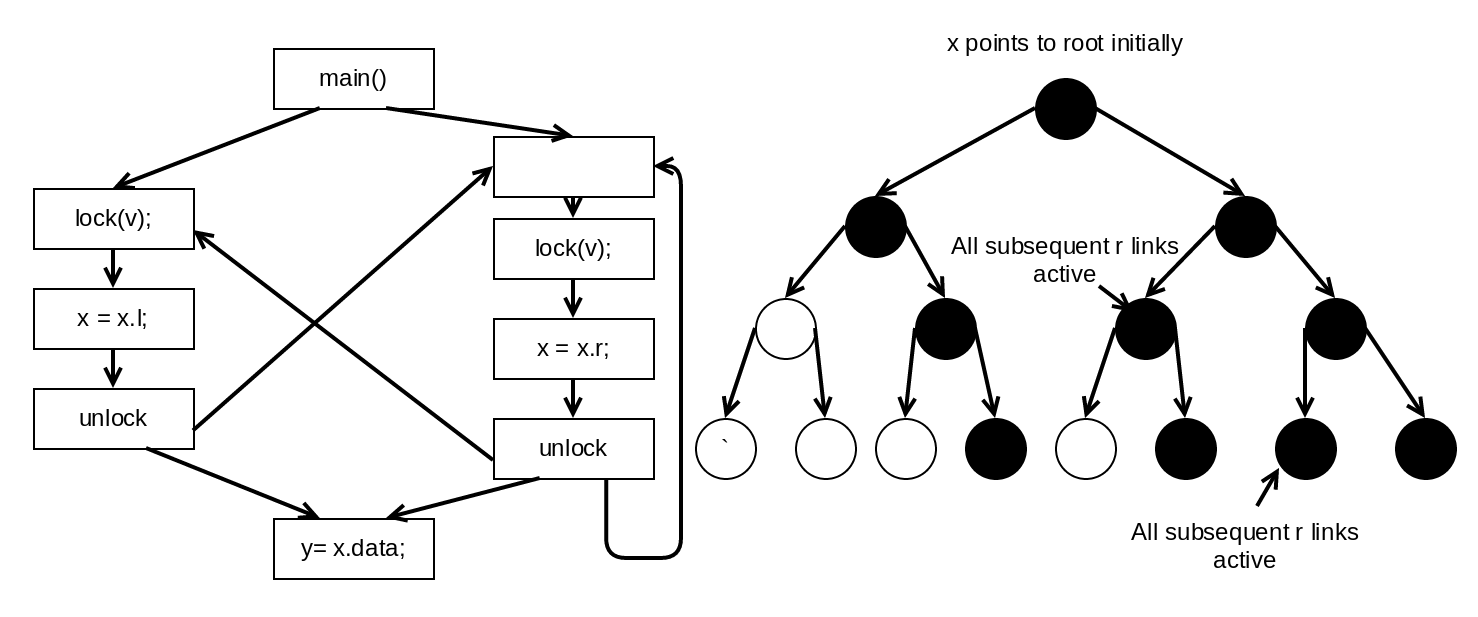
\includegraphics[width=0.8\textwidth]{Figures/tree3.png}
	\caption{Another Concurrent access example in a tree}
	\label{fig:ch5example}
\end{figure}

Another interesting example is the case when both the loops are outside critical sections in Figure 6.5. This will lead to any number of executions of $C_1$ and $C_2$ and interleaving are also possible. Thus the access graph expected for this kind of execution is \emph{x.\{l\textsuperscript{*}.r\textsuperscript{*}\}\textsuperscript{*}} . Starting with $C_1$, either multiple executions of $C_1$ and $C_2$ are possible. Also there is no restriction on the thread switchings. So for this example, all the nodes of the tree can be live/accessed. \\

\begin{figure}
	\centering
	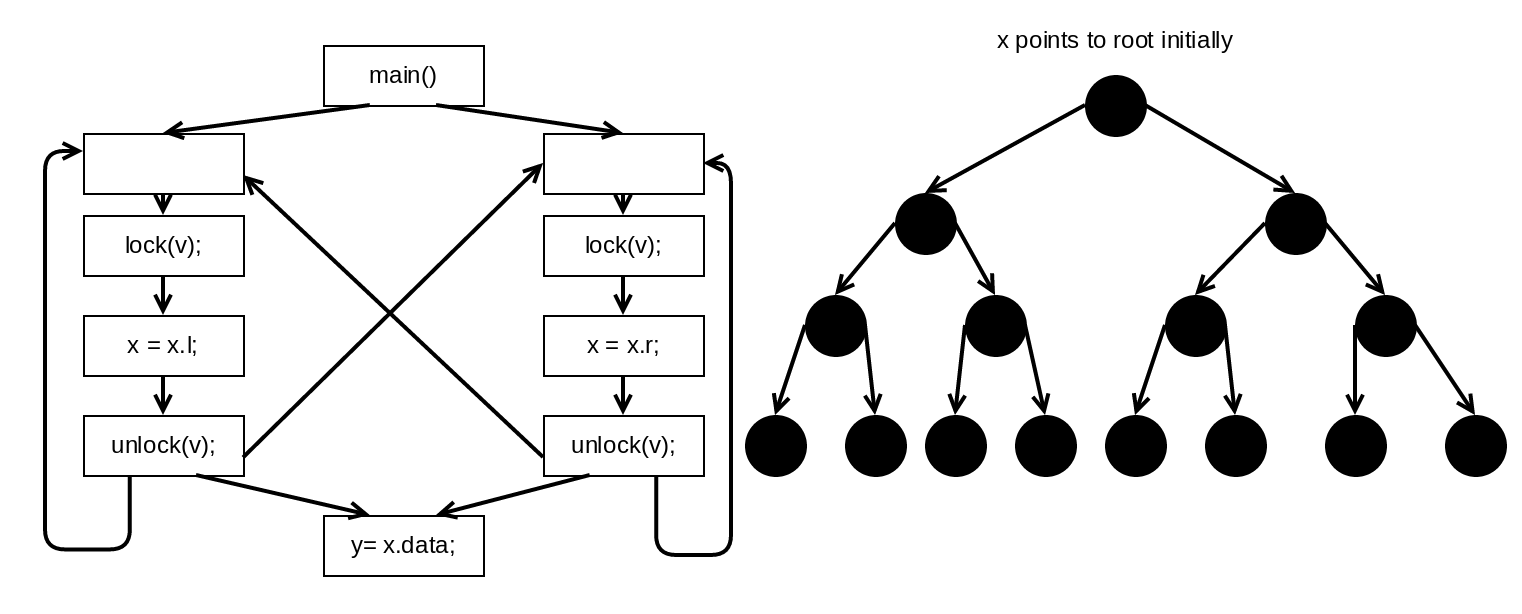
\includegraphics[width=0.8\textwidth]{Figures/tree4.png}
	\caption{Another Concurrent access example in a tree}
	\label{fig:ch5example}
\end{figure}

From all these examples, we can think of a way to propagate data flow values/access graphs across the synchronized control flow graph. We would have $n$ starting points , where $n$ is the number of threads in the program. Starting from a thread, data flow values are propagated along valid execution sequences. A valid execution sequence is such that all the thread switchings are consistent. This is ensured by examining all the critical sections. In a valid execution sequence, critical sections with no loops outside it appear only once. \\

For instance, in Figure 6.2 execution sequences possible are $T_1$,$T_2$ or $T_2$,$T_1$. We can also write this in terms of execution over critical sections. For this we will first need to run an analysis on each thread locally and find out the critical section(s) present. After identification, we also need to figure out whether the critical sections can be executed once or any number of times. Once we have the results from the intra-thread analysis, we will add the inter-thread edges to generate execution sequence over critical sections. \\

For example